\documentclass{beamer}
\usepackage[utf8]{inputenc}
\usepackage[slovak]{babel}
\usepackage{graphicx}
\usepackage{enumerate}

\usetheme{CambridgeUS}

\author{Adrián Tomašov \\ xtomas32}
\title{Virtuálne switche/bridge v linuxe}


\begin{document}

%uvodny frame
	\begin{frame}
		\titlepage
	\end{frame}

%obsah
	\begin{frame}{Obsah}
		\begin{itemize}
			\item{Úvod}
			\item{Linux bridge}
			\item{Open virtual switch}
		\end{itemize}
	\end{frame}
	
	
%uvod
	\begin{frame}{Úvod}
		Využitie switchov
		\begin{itemize}
			\item{pripojenie virtuánych strojov medzi sebou}
			\item{spojenie virtuálnej siete s fyzickou sieťou}
			\item{logické rozdelenie fyzickej siete (vlan, vxlan)}
			\item{základ takmer každej cloud infraštruktúry}
		\end{itemize}
		
		\begin{figure}
			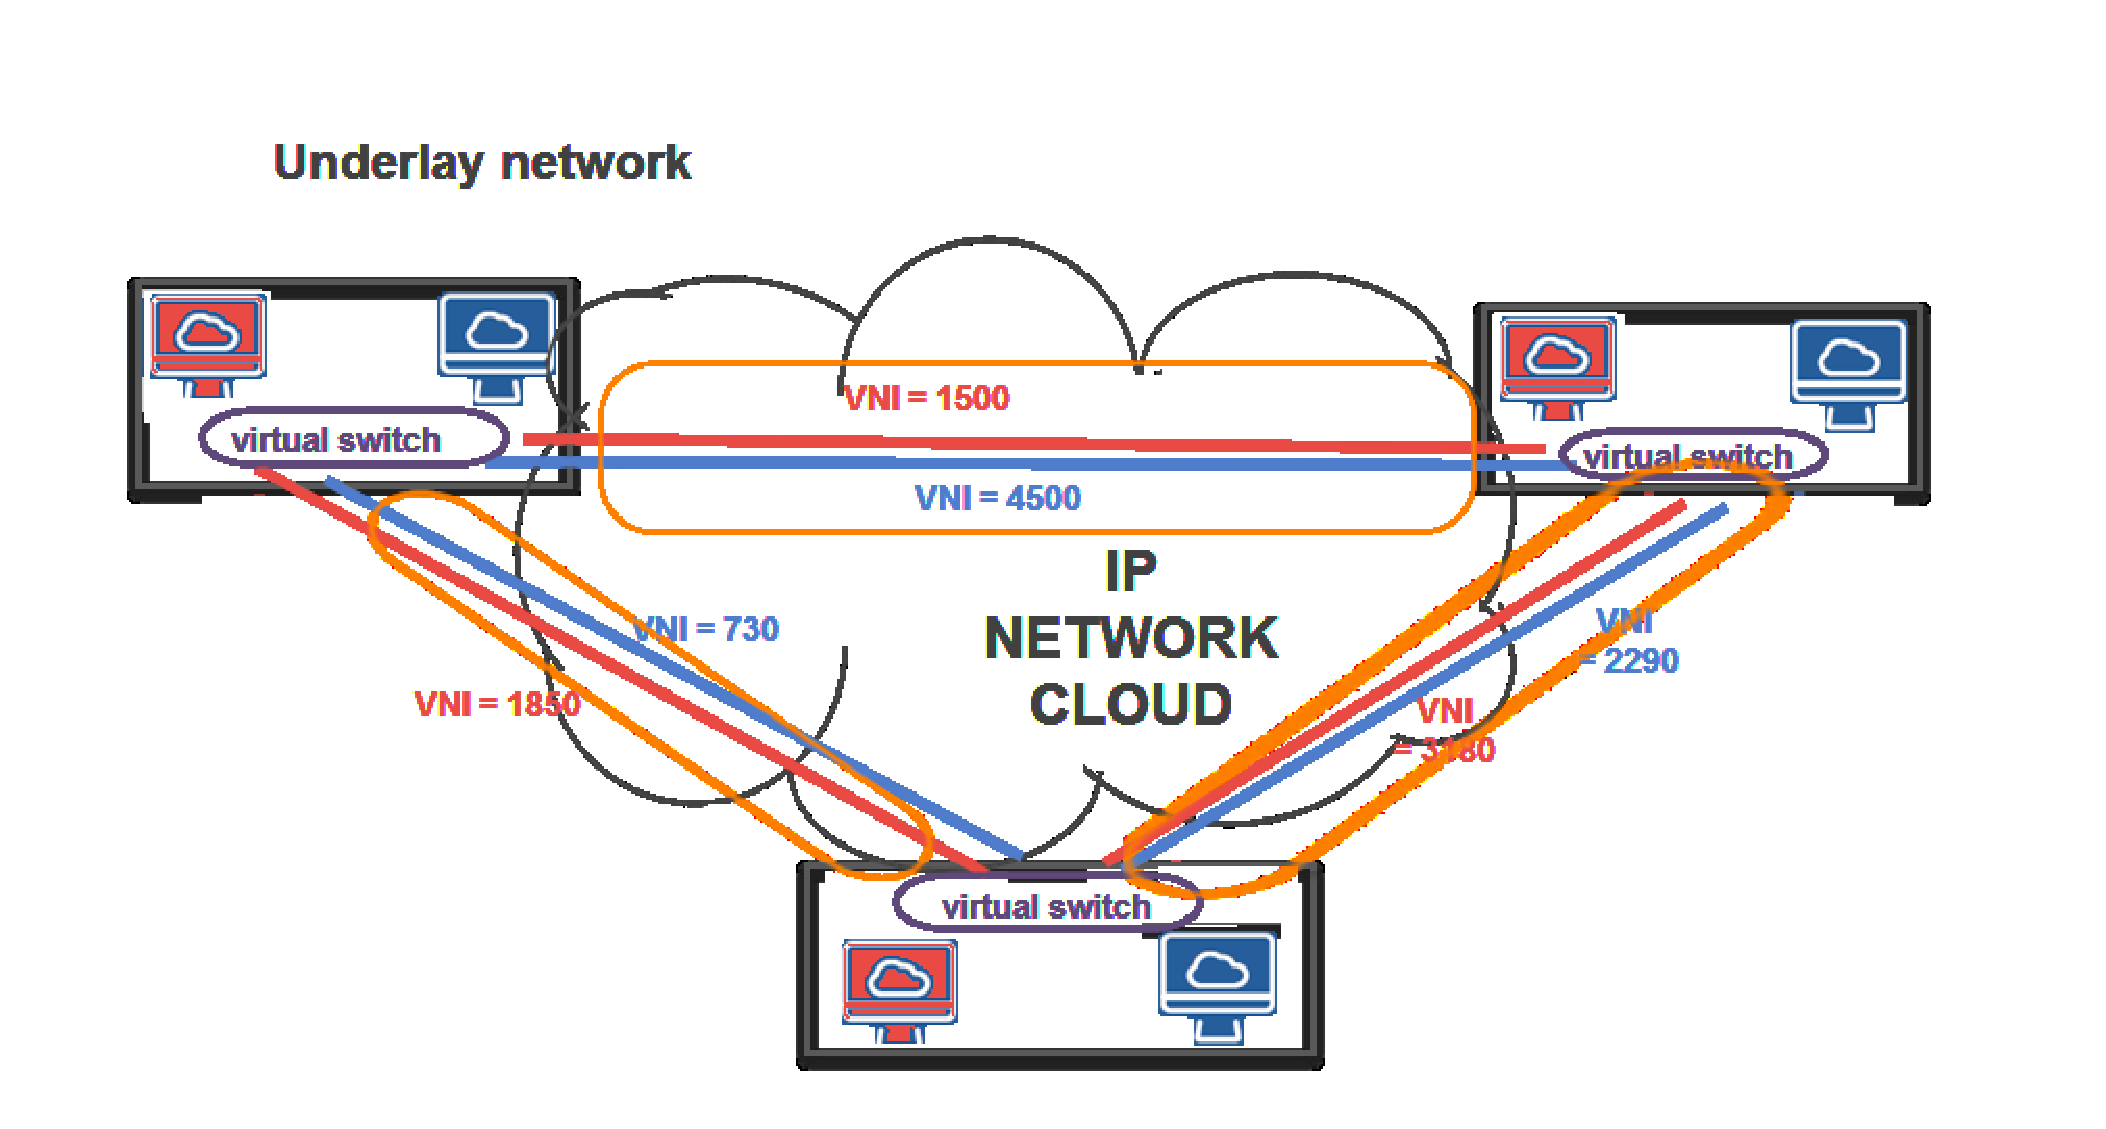
\includegraphics[scale=0.2]{Underlay-final-1.eps}
			\caption{Príklad cloud infraštruktúry}
		\end{figure}
	\end{frame}

%realny priklad
	\begin{frame}{Reálny príklad používania}
		\begin{figure}
		
			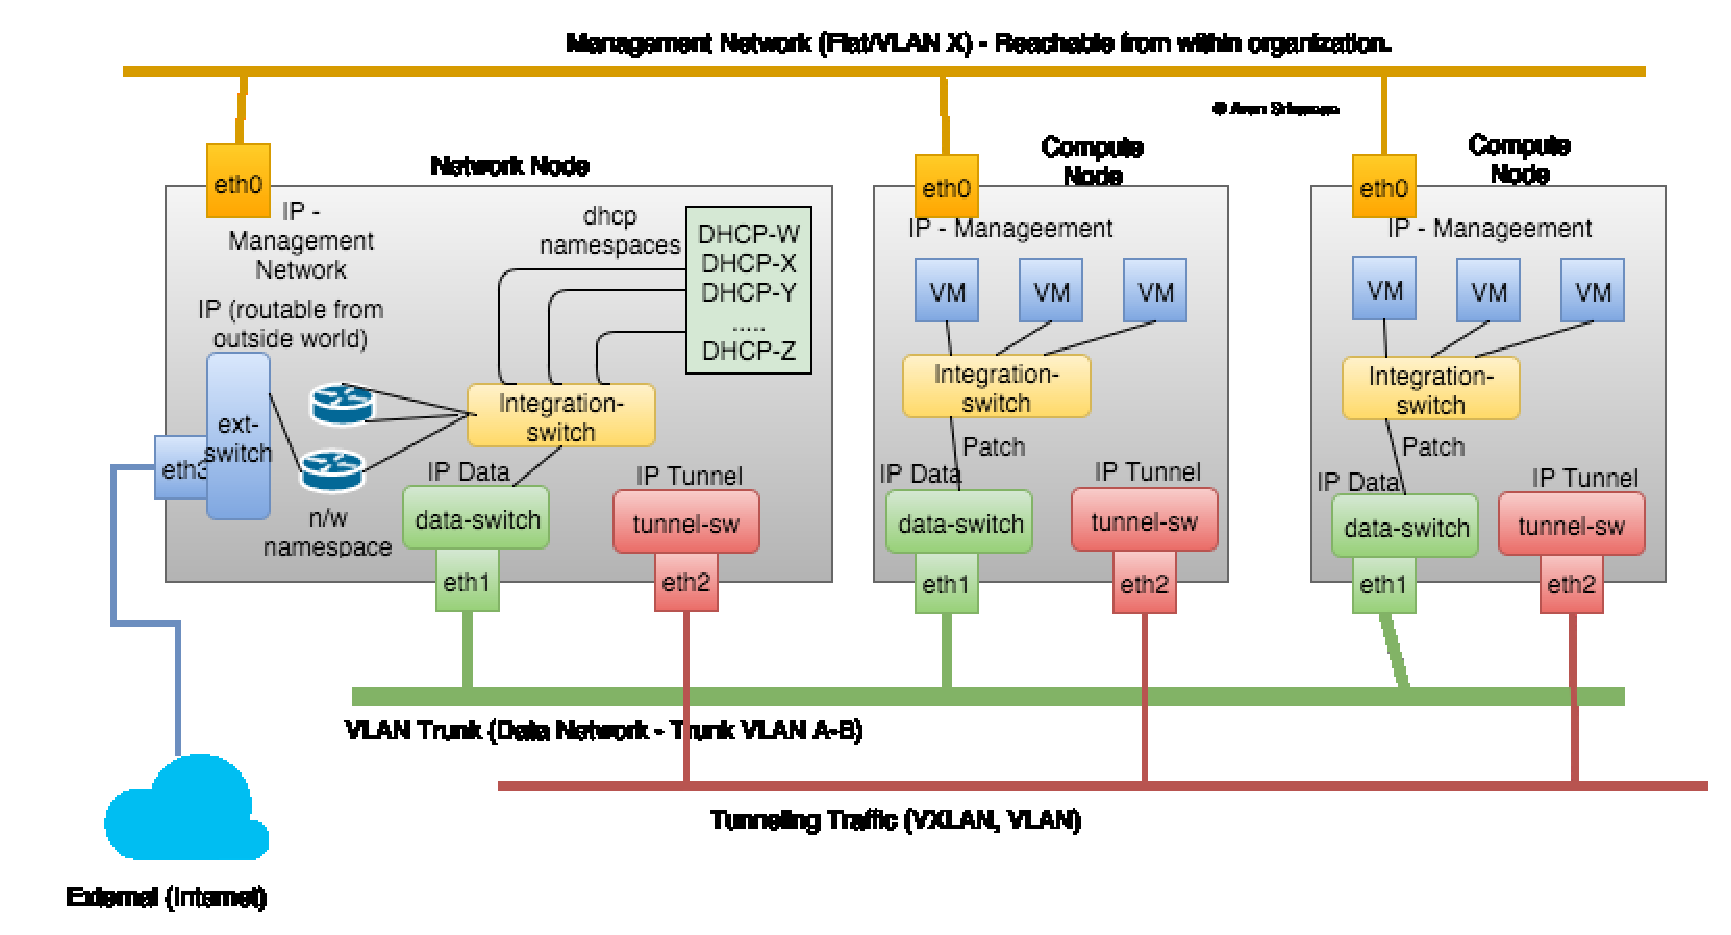
\includegraphics[scale=0.4]{private-cloud.eps}
			\caption{Zapojenie serverov, na ktorých sú spustené virtuálne stroje so zapojením do virtuálnych switchov}
		\end{figure}
	\end{frame}

%linux brigde
	\begin{frame}{Linux bridge}
		\begin{itemize}
			\item{balík bridge-utils}
			\item{prvý krát použitý v kerneli 2.2 a integrovaný do kernelov 2.4 a 2.6}
			\item{preposiela na základe druhej vrstvy osi modelu (L2 switch)}
			\item{plug and play}
		\end{itemize}
	\end{frame}

%linux bridge vyhody
	\begin{frame}{Linux bridge výhody/nevýhody}
		Výhody
		\begin{itemize}
			\item{filtovanie trafiky}
			\item{podpora STP protokolu}
			\item{podpora IGMP snooping}
		\end{itemize}
		Nevýhody
		\begin{itemize}
			\item{pomalší v porovnani s open virtual switchom}
			\item{nepodporuje VXLAN}
		\end{itemize}
	\end{frame}

%ovs 
	\begin{frame}{Open vSwitch}

%		\begin{minipage}{0.6\textwidth}
%				\includegraphics[scale=0.2]{vswitch.eps}	
%		\end{minipage}

		\begin{columns}

		\column{0.8\textwidth}
				\begin{itemize}
					\item{Feb 27 2017: Open vSwitch 2.7.0}
					\item{licencia open source Apache2.0}
					\item{navrhnutý pre veľké produkčné prostredia}
					\item{podporuje automatizovanú správu (OVSDB mgmt. protocol, OpenFlow)}
					\item{podporuje viacero fyzických serverov podobných VMware's vNetwork alebo Cisco Nexus 1000V}
				\end{itemize}
		

		\column{0.2\textwidth}
				\includegraphics[scale=0.35]{vswitch.eps}	
		\end{columns}


	\end{frame}

%OVS vyhody / nevyhody
	\begin{frame}{Open vSwitch výhody/nevýhody}
		Výhody
		\begin{itemize}
			\item{podporuje viacero tunelovacích protokolov (GRE, VXLAN, STT, and Geneve s podporou IPsec)}
			\item{monitorovanie trafiky pomocou SPAN, RSPAN, a pod.}
			\item{podpora DPDK}
		\end{itemize}
		
		Nevýhody
		\begin{itemize}
			\item{nepodporuje iptables}		
		\end{itemize}
	\end{frame}

%porovnanie
	\begin{frame}{Porovnanie}
		por
	\end{frame}

%zdroje
	\begin{frame}{Zdroje}
		\begin{itemize}
			\item{http://openvswitch.org/}
			\item{https://wiki.archlinux.org/index.php/Network\_bridge}
			\item{http://blog.arunsriraman.com/2015/12/running\-vlan-vxlan-and-gre-together.html}
			\item{http://www.stratoscale.com/blog/networking/network-virtualization-overlay-networks-cloud-environments-part-2/}
		\end{itemize}
	\end{frame}
	
	\begin{frame}
	\begin{center}
		Ďakujem za pozornosť
	\end{center}
	\end{frame}

\end{document}
